\chapter{Introduction}
\label{chap:introduction}
\setcounter{page}{1}
\pagenumbering{arabic}

In recent years, computer vision has made great progress. People have achieved good results in some simple tasks and have been applied in many fields, such as image classification~\cite{yu2017convolutional, lu2007survey}, image segmentation ~\cite{pham2000current} and face recognition~\cite{ahonen2006face, phillips1996feret}. Now people are no longer satisfied with these basic tasks, but hope that computers can interpret pictures like humans to obtain more information, such as the attributes of objects,  the motion of objects, and the relationships between objects, etc. Thus people began to study some complex tasks such as mage Captioning ~\cite{hossain2019comprehensive},  Visual Question Answer~\cite{antol2015vqa}, and  visual relationship detection (VRD). \\

\begin{figure}[!htbp]
	\centering
	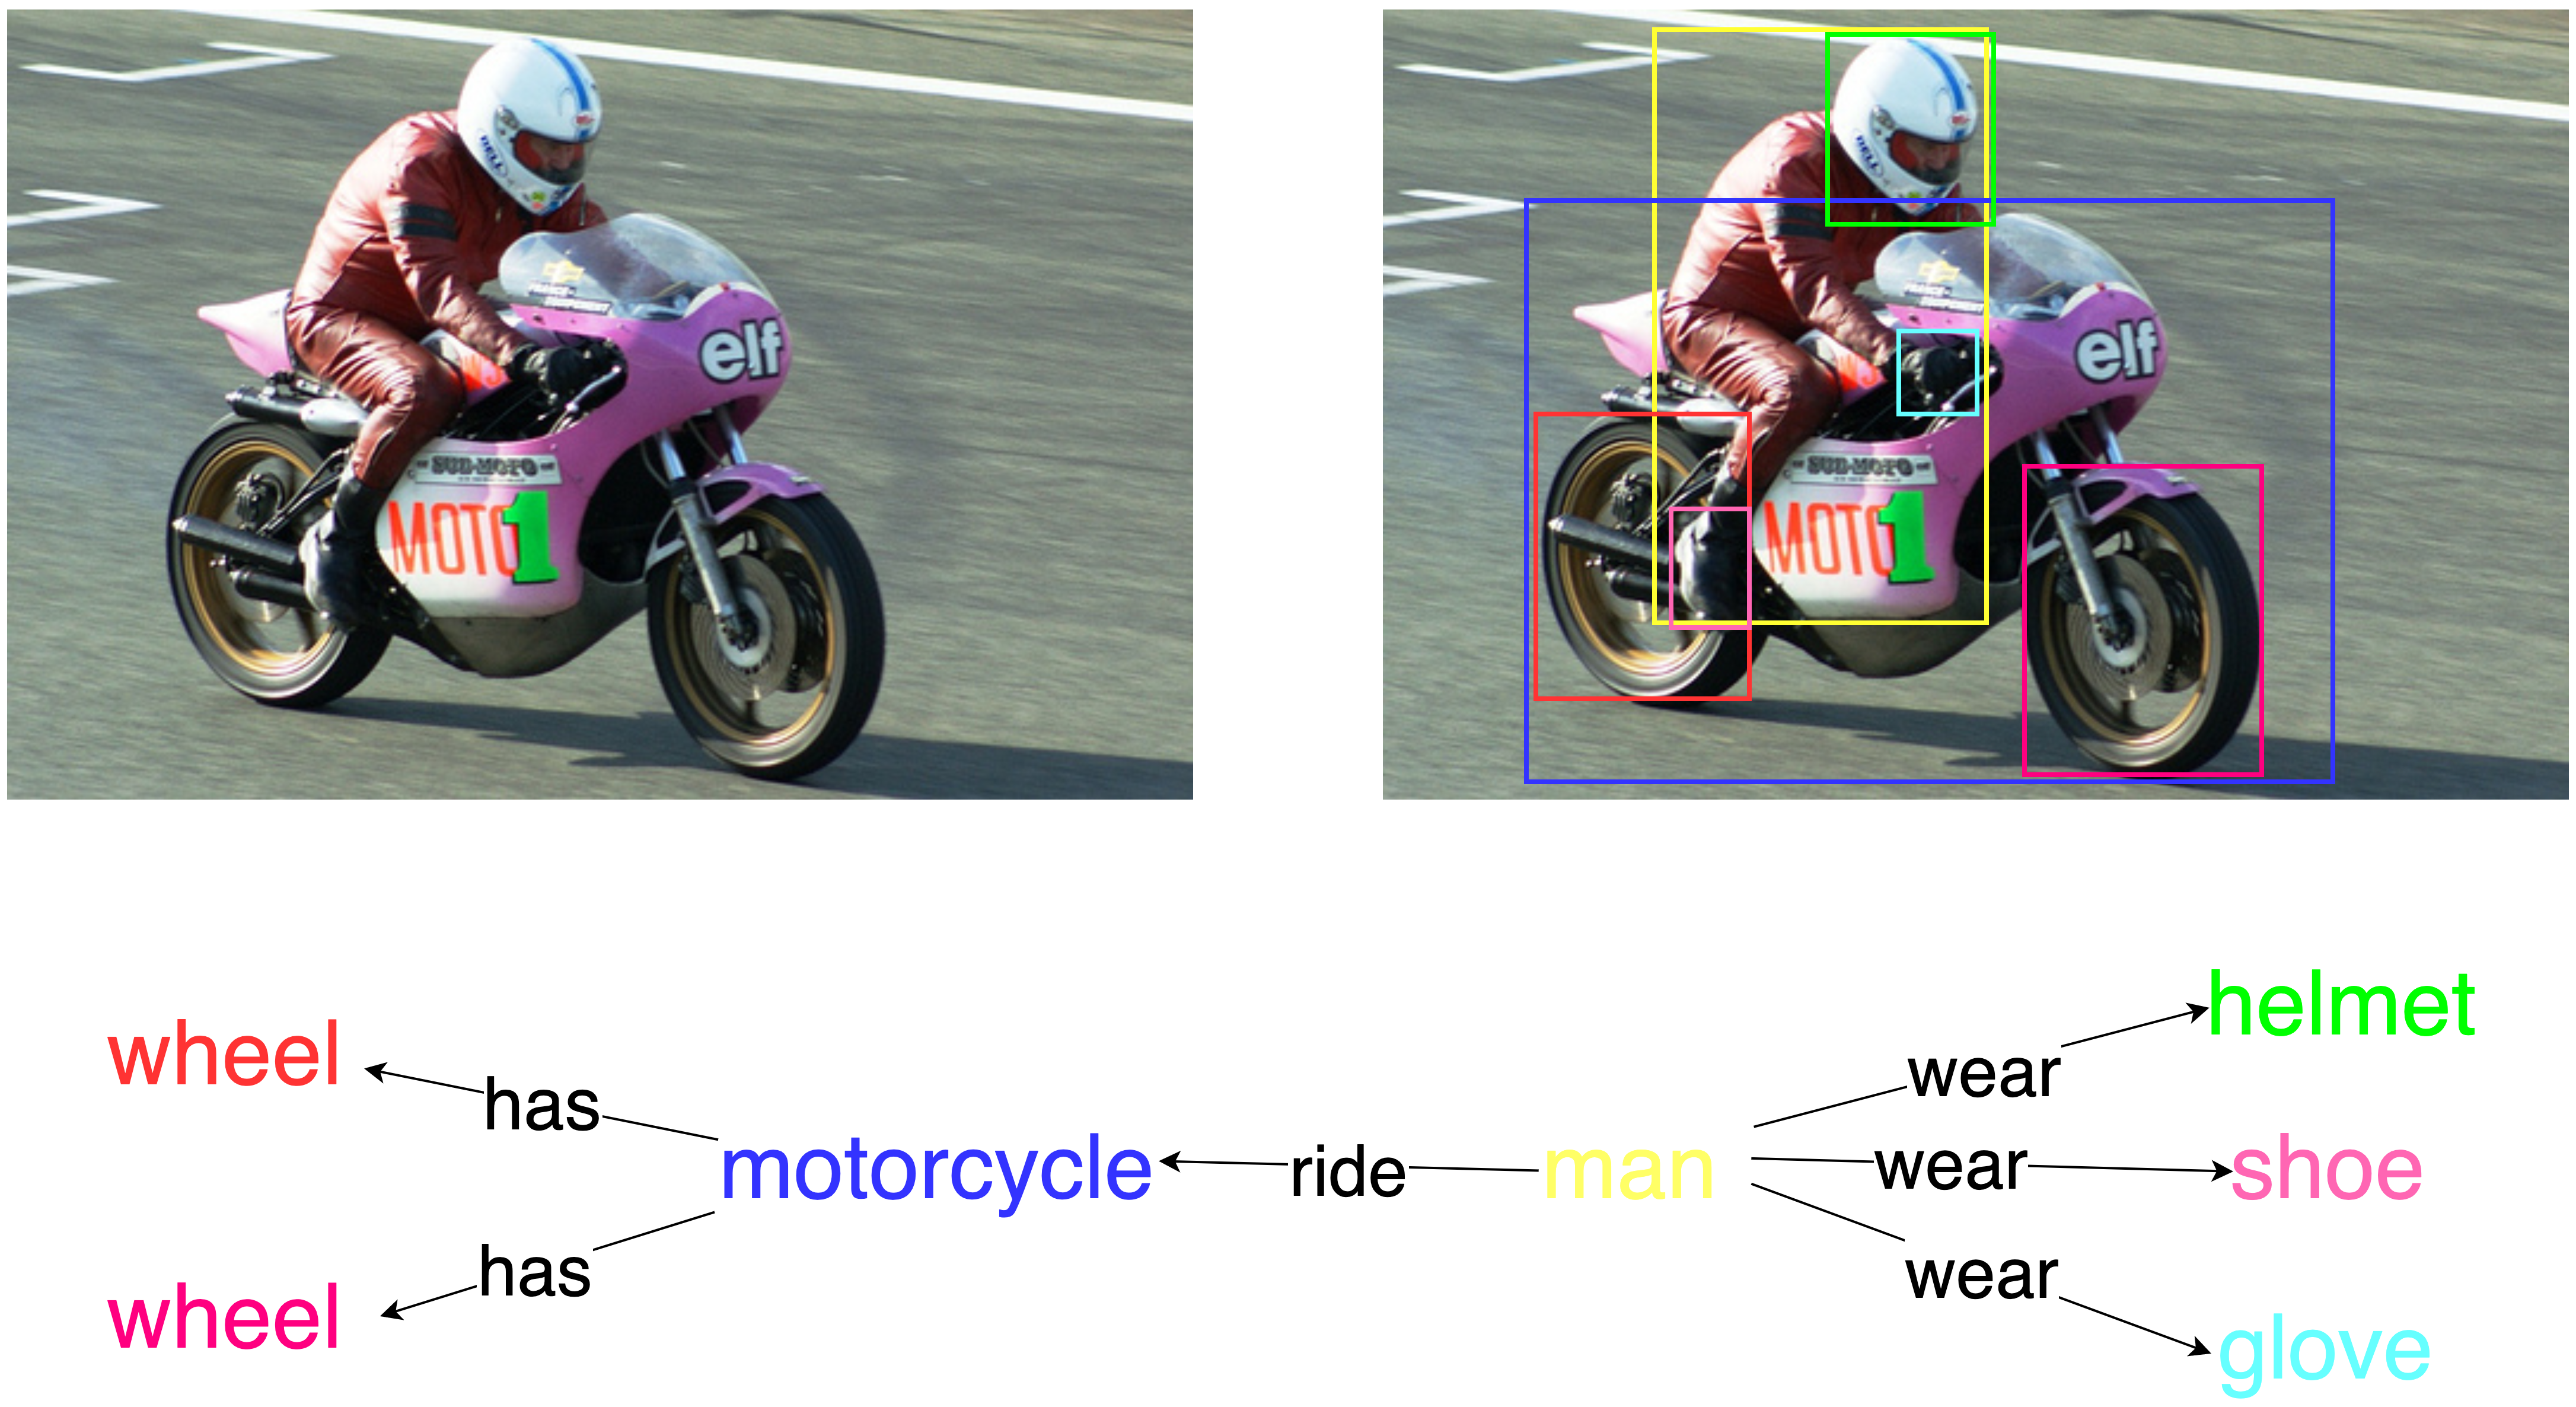
\includegraphics[width = 0.9 \textwidth]{figures/senen_graph.png}
	\caption[A example of visual relationship detection]
	{ A example of visual relationship detection: The upper left corner is the original input image, the upper right corner is the result of object detection, and the lower one is the relationship detection}
	\label{fig:sene}
\end{figure}

The visual relationship detection task not only needs to recognize the objects in the image and their positions, but also recognize the relationship between the objects, that is, the connection between the target objects, which can be expressed as a triplet-Relationship: $\left \langle subject, predicate, object\right \rangle$. For example, in figure~\ref{fig:sene}, a VRD task includes identifying instances in the image: motorcycle, man, helmet, wheels, etc., as well as identifying the relationship between them, like $\left \langle man, ride, motorcycle\right \rangle$, $\left \langle man, wear, helmet\right \rangle$, $\left \langle motor, has, wheel\right \rangle$, etc..




\section{Motivation}

Visual relationship detection connects objects in images with predicates, and also connects low-level vision and high-level language (see Figure ~\ref{fig:vrd}). This means that visual relationship detection can provide high-level tasks, such as image subtitles [7] for easier-to-understand information; it can also improve low-level tasks such as object detection using scene context. Visual relationship detection is an essential step to realize that computers can understand images as intelligently as humans.

\begin{figure}[!htbp]
	\centering
	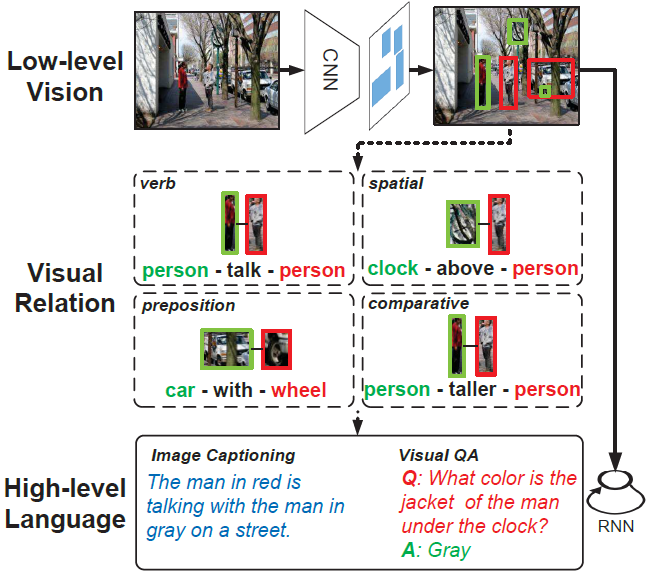
\includegraphics[width = 0.9 \textwidth]{figures/VRD.png}
	\caption[Connection between low-level vision and high-level vision]
	{ Visual relationship detection understands object interactions directly, which offer further semantic information for applications such as image captioning and QA. Figure obtained from ~\cite{zhang2017visual}}
	\label{fig:vrd}
\end{figure}

In recent years, with the proposal of the Transformer structure~\cite{vaswani2017attention}(see in section~\ref{section:transformer}), people have found that it not only achieves excellent performance in natural language processing tasks, but also has a very wide range of applications in computer vision, such as the DETR model~\cite{carion2020end} (see Figure ~\ref{fig:detr})proposed by Nicolas et al., using the Encoder-Decoder structure of the Transformer, The object detection effect of DETR is not inferior to Faster R-CNN~\cite{ren2016faster}. Thus we want to study the possibility of transformer structure in VRD problem.

\begin{figure}[!htbp]
	\centering
	\includegraphics[width = 1 \textwidth]{figures/DETR.png}
	\caption[The framework of DETR model]
	{ The framework of DETR model. Figure obtained from ~\cite{carion2020end}}
	\label{fig:detr}
\end{figure}


There are three main related tasks of visual relationship detection task: Predicate classification, which only needs to predict the relationship. Scene graph classification needs to get objects and relationships. Scene graph detection/gen also needs to locate the objects and relationships of the box.

The challenges for our task are mainly summarized as follows:

\begin{enumerate}[\qquad  1.]
	\item Try to apply the transformer structure to the VRD problem.
	\item The DETR model use learned embedding vectors as object queries, which has poor interpretability . so we encode the known information to replace the fixed small set of learned object queries in DETR.
	\item  The object features in DETR model can be visualized through the attention map, so we try to use the attention map to visualize the relationship features.
	\item  Explore the impact of different queries on the model 
\end{enumerate}

Firstly,  in an image it is important to understand the role of each object and how objects are related and influenced by others in the context of the whole image.

Secondly, the most important challenge is to predict correct predicates, describing the relationship among two objects. 
 

\section{Contribution}

In this thesis, we provide  an efficient framework based on Encoder-Decoder of the  Transformer structure  for visual relationship detection that detects the interactions between objects in the image. The main work and contributions are summarized as following:
\begin{enumerate}[\qquad  1.]
	\item Introduce a new framework to solve the VRD problem base on the transformer.
	\item Propose new object feature extraction methods and context methods.
\end{enumerate}


\section{Organization of the Thesis}
This thesis is structured as follows:

In Chapter~\ref{chap:relatedwork} , we will discuss about the related works. Some advanced researches and models about object detection and visual relationship detection are introduced briefly. We also demonstrate their contributions and limitations.

In Chapter ~\ref{chap:bg}, the theories about Transformer and other important models and algorithm such as Faster R-CNN , Hungarian matching and ranking loss  will be introduced.

In Chapter ~\ref{chap:framework}, the proposed framework will be shown in detail.

In Chapter ~\ref{chap:experiment}, the experimental results will be presented and analyzed in detail. Our proposed framework are evaluated on Visual Genome with three standard evaluation metrics.

In Chapter ~\ref{chap:conclusion}, we conclude our work finally and point out the future research direction.